% !TEX encoding = UTF-8 Unicode
%%% LaTeX Template: Curriculum Vitae
%%%
%%% Source: http://www.howtotex.com/
%%% Feel free to distribute this template, but please keep the referal to HowToTeX.com.
%%% Date: July 2011

%%% ------------------------------------------------------------
%%% BEGIN PREAMBLE
%%% ------------------------------------------------------------
\documentclass[paper=a4,fontsize=11pt]{scrartcl}	 			% KOMA-article class							
%\usepackage[english]{babel}								% English language/hyphenation
\usepackage[usenames,dvipsnames,svgnames,table]{xcolor}
%\color{darkgray}
\usepackage{framed,color}
%\definecolor{shader}{rgb}{1,0.8,0.3}
%\definecolor{shader}{rgb}{1,1,1}
%\definecolor{black}{black}{0.25}
%\usepackage[protrusion=true,expansion=true]{microtype}		% Better typography
\usepackage{amsmath,amsfonts,amsthm}					% Math packages
\usepackage{graphicx}								% Enable pdflatex
\usepackage[svgnames]{xcolor}							% Colors by their 'svgnames'
\usepackage[left=2cm,top=1cm,right=2cm,bottom=2cm,nohead,nofoot]{geometry}									% Saving trees ;-) 
%\usepackage{url}
\usepackage{hyperref}										% Clickable URL's
\usepackage{wrapfig}									% Wrap text along figures
\usepackage{comment}
\renewcommand{\refname}{PUBLICATIONS}
% Bibliography
\usepackage{natbib}
%\usepackage[sorting=ydnt]{biblatex}
\usepackage{bibentry}
%\usepackage{bibtex}
%\nobibliography*
\bibliographystyle{apa}

%%add a picture
%\graphicspath{ {images/} }
%\DeclareGraphicsExtensions{.jpg,.pdf,.png}



%%% Chinese typesetting %%%%%%%%%%%
%\usepackage{xeCJK}
%\setCJKmainfont{STFangsong}
%\XeTeXlinebreaklocale "zh" 
%\XeTeXlinebreakskip = 0pt plus 1pt

\frenchspacing									% Better looking spacings after periods
\pagestyle{empty}								% No pagenumbers/headers/footers
%\usepackage{bbding}									% Symbols


%%% Custom sectioning (sectsty package)
%%% ------------------------------------------------------------
\usepackage{sectsty}							% Custom sectioning (see below)

\sectionfont{%									% Change font of \section command
	\usefont{OT1}{phv}{b}{n}%					% bch-b-n: CharterBT-Bold font
	\sectionrule{0pt}{0pt}{-5pt}{3pt}
	}

%%% Macros
%%% ------------------------------------------------------------
\newlength{\spacebox}
\settowidth{\spacebox}{8888888888}				% Box to align text
\newcommand{\sepspace}{\vspace*{1em}}			% Vertical space macro

\newcommand{\MyName}[1]{
		\Huge \usefont{OT1}{phv}{b}{n} \hfill #1 		% Name
		\par \normalsize \normalfont}
		
\newcommand{\MySlogan}[1]{
		\large \usefont{OT1}{phv}{m}{n}\hfill \textit{#1} % Slogan (optional)
		\par \normalsize \normalfont}

\newcommand{\NewPart}[1]{\section*{\uppercase{#1}}}

\newcommand{\PersonalEntry}[2]{
		\noindent\hangindent=2em\hangafter=0 		% Indentation
		\parbox{\spacebox}{						% Box to align text
		\textit{#1}}								% Entry name (birth, address, etc.)
		\hspace{1.5em} #2 \par}					% Entry value

\newcommand{\SkillsEntry}[2]{						% Same as \PersonalEntry
		\noindent\hangindent=2em\hangafter=0 		% Indentation
		\parbox{\spacebox}{						% Box to align text
		\textit{#1}}								% Entry name (birth, address, etc.)
		\hspace{1.5em} #2 \par}					% Entry value	
		
\newcommand{\EducationEntry}[4]{
		\noindent \textbf{#1} \hfill 					% Study
		\colorbox{White}{%
			\parbox{10em}{%
			\hfill\color{Black}#2}} \par				% Duration
		\noindent \textit{#3} \par					% School
		\noindent\hangindent=2em\hangafter=0 \small #4 	% Description
		\normalsize \par}

\newcommand{\WorkEntry}[4]{						% Same as \EducationEntry
		\noindent \textbf{#1} \hfill 					% Jobname
		\colorbox{White}{\color{Black}#2} \par		% Duration
		\noindent \textit{#3} \par					% Company
		\noindent\hangindent=2em\hangafter=0 \small #4 	% Description
		\normalsize \par}
\newcommand{\RefEntry}[7]{						% Same as \EducationEntry
		\noindent \textbf{#1} \par 					% Jobname
		\noindent \textit{#2} \par	% Duration
		\noindent \textit{#3} \par
		\noindent \textit{#4} \par% Company 	% Description
		\noindent \textit{#5} \par
		\noindent \textit{#6} \par
		\noindent \textit{#7} \par
		}

\newcommand{\ServiceEntry}[2]{					% Same as \EducationEntry
		\noindent \textit{#1} \par					% Company
		\noindent\hangindent=2em\hangafter=0 \small #2 	% Description
		\normalsize \par}
\newcommand{\codeEntry}[2]{						% Same as \EducationEntry
		\noindent \textbf{#1} \hfill 					% Jobname
		\colorbox{White}{\color{Black}#2} \par		% Duration
		%\noindent \textit{#2} \par					% Company
		%\noindent\hangindent=2em\hangafter=0 \small #4 	% Description
		%\normalsize \par}
		}
		
\def\FormatName#1{%
  \def\myname{Simon Renny-Byfield}%
  \edef\name{#1}%
  \ifx\name\myname
    \textbf{#1}%
  \else
    #1%
  \fi
}

%%% ------------------------------------------------------------
%%% BEGIN DOCUMENT
%%% ------------------------------------------------------------
\begin{document}
%\bibliographystyle{nature}
%\bibliographystyle{apalike}
%\bibliographystyle{mystyle}
%\begin{comment}
%\begin{wrapfigure}{l}{0.5\textwidth}
%	\vspace*{-2em}
%		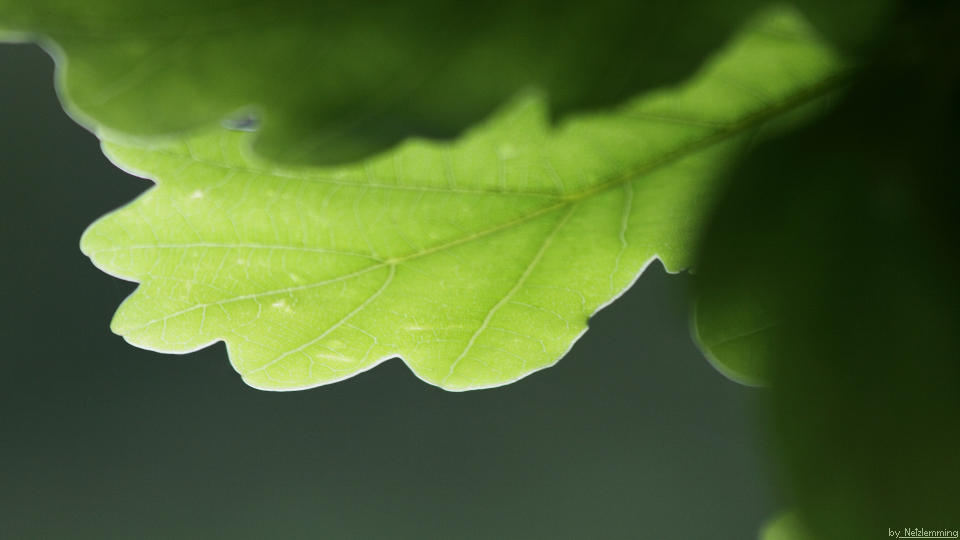
\includegraphics[width=0.15\textwidth]{photo}
%\end{wrapfigure}
%\end{comment}

%\begin{shaded}\color{shader}\MyName{Simon\color{gray}Renny-Byfield}\end{shaded}
\MyName{Simon \color{gray}Renny-Byfield}
%\MySlogan{\textit{Try not to become a man of success but a man of value.}}
%\MySlogan{\textit{---- Albert Einstein}}
\color{black}
\sepspace

%%% Personal details
%%% ------------------------------------------------------------
\NewPart{Personal details}{}
%\includegraphics{myphoto.jpg}
%\PersonalEntry{Birth}{December 20, 1986} 
\begin{minipage}{0.6\textwidth}\raggedright
\PersonalEntry{Address}{Department of Plant Sciences}
\PersonalEntry{}{Robbins Hall}
\PersonalEntry{}{University of California, Davis}
\PersonalEntry{}{California, USA, 95616}
\PersonalEntry{Mobile}{(515) 509-3184}
\PersonalEntry{E-Mail}{\href{mailto:sbyfield@ucdavis.edu}{\color{blue}{sbyfield@ucdavis.edu}}}
%\PersonalEntry{Website}{www.githubZZZ.com}
\end{minipage}
\begin{minipage}{0.3\textwidth}\raggedleft% adapt widths of minipages to your needs
%\includegraphics[scale=0.025]{myphoto}
\end{minipage}
%\PersonalEntry{Webpage}{\href{https://wiki.qut.edu.au/display/cyphy/Hu+He}{\color{red}{https://wiki.qut.edu.au/display/cyphy/Hu+He}}}
%\PersonalEntry{}{\href{http://hehuvision.blogspot.com}{\color{red}{http://hehuvision.blogspot.com}}}

%%% Education %%%%%
%%% ------------------------------------------------------------
\NewPart{Academic Qualifications}{} 

\EducationEntry{Ph.D. Plant Evolutionary Genomics}{2008-2012}{Queen Mary University of London, UK}{Supervisors: Professor Andrew R. Leitch\\
Thesis Title: Evolution of repetitive DNA in angiosperms: Examples from \textit{Nicotiana}}
\sepspace

\EducationEntry{B.Sc Genetics First Class Honors}{2005-2008}{Queen Mary University of London, UK}

\NewPart{Professional Experience}{}

\WorkEntry{Post-Doctoral Research}{University of California, Davis}{Supervisor: Dr. Jeffrey Ross-Ibarra}{2014-present}
\WorkEntry{Post-Doctoral Research}{Iowa State University}{Supervisor: Prof. Jonathan F. Wendel}{2012-2014}
%\WorkEntry{Post-Doctoral Research}{Queen Mary University of London}{Supervisor: Prof. Andrew R. Leitch}{2012}

%\NewPart{Publications}{}
%\renewcommand\refname{\vskip -1cm}
%\bibliographystyle{siam}
\nocite{*}
\bibliography{cv.template}
\bibliographystyle{plain}
%\printbibliography

\vspace{7 mm}
\text{\textsuperscript{\dag} joint first author}

\NewPart{Teaching}{}
\WorkEntry{Teaching Assistant}{Queen Mary University of London}{Chromosomal and Population Genomics}{2008-2012}
\WorkEntry{Teaching Assistant}{Queen Mary University of London}{Undergraduate Thesis Advisor}{2008-2012}
\WorkEntry{Guest Lecturer}{Queen Mary University of London}{MSc Research Seminar}{2012}
%\WorkEntry{Guest Lecturer and Teaching Assistant}{University of California, Davis}{Ecological Genomics}{2015}

\NewPart{Awards and Grants}{}
\WorkEntry{PhD Fellowship}{Natural Environment Research Council via Queen Mary University of London}{\textsterling{18,000} \textit{per annum} stipend and consumables}{2008-2012}
\WorkEntry{Extra Consumables}{Queen Mary University of London}{\textsterling{4000}}{2008-2012}
\WorkEntry{Bevan Prize}{Queen Mary University of London}{Outstanding Academic achievement in Genetics}{2008}
\WorkEntry{Irene Manton Prize}{Linnean Society of London}{Best Ph.D in Botany}{2014}
\NewPart{Coding and High Performance Computing}
\codeEntry{Perl}{Advanced}
\codeEntry{R}{Advanced}
\codeEntry{Bash}{Proficient}
\codeEntry{High Performance Computing}{Proficient}
\NewPart{Peer review}{}
Heredity\\
BMC Genomics\\
PLOS One\\
Botanical Journal of the Linnean Society\\
BMC Plant Biology\\
New Phytologist

\NewPart{References}
%\address{42 Apartment complex}{Street}{City\\Country}
\RefEntry{Dr. Jeffrey Ross-Ibarra}{University of California, Davis}{Department of Plant Sciences}{Robbins Hall}{Davis CA, 95616}{rossibarra@ucdavis.edu}{530-752-1152\\}
\RefEntry{Prof. Jonathan F. Wendel}{Iowa State University}{Department of Ecology, Evolution and Organismal Biology}{Bessey Hall}{Ames IA, 50010}{jfw@iastate.edu}{(515) 294-717\\}
\RefEntry{Prof. Andrew R. Leitch}{Queen Mary University of London}{Fogg Building}{School of Biological and Chemical Sciences}{London UK, E1 4NS}{a.r.leitch@qmul.ac.uk}{+44 (0)20 7882 6483\\}
%\WorkEntry{Post-Doctoral Research}{Queen Mary University of London}{Supervisor: Prof. Andrew R. Leitch}{2012}
%%% Publications
%%% ------------------------------------------------------------
%\NewPart{Publications}{}
%\begin{enumerate}
%\item \bibentry{he2012measuring}
%\item \bibentry{he2011towards}
%\item \bibentry{he2010graphcut}
%\item \bibentry{mckinnon2011towards}
%\item \bibentry{warren2012large}
%\item \bibentry{warren2010unaided}
%\end{enumerate}
%
%{\color{red}{\textit{Manuscripts under Review}:}}
%\begin{enumerate}
%\item \bibentry{hu2013ietcv}
%\item \bibentry{hu2013sensors}
%\item \bibentry{hu2013aim}
%\item \bibentry{hu2013IROS}
%\item \bibentry{inkyu2013aim}
%\item \bibentry{Ferrari2013mee}
%\end{enumerate}
%
%
%%%% Work experience
%%%% ------------------------------------------------------------
%\NewPart{Experience}{}
%\WorkEntry{Teaching Assistant}{Mar 2012 - Jul 2012}{Queensland University of Technology}{\textbf{ENB244} Microprocessors and Digital Systems}
%\sepspace
%\WorkEntry{Research Assistant}{Aug 2009 - Dec 2010}{The University of Queensland}{Working for CRCMining on multiple sensors fusion using EKF}
%\sepspace
%\WorkEntry{Teaching Assistant}{Mar 2010 - Dec 2010}{The University of Queensland}{\textbf{MECH3750} Numerical Analysis and Python Programming\\
%\textbf{MECH2301/2300} Structure Mechanics}
%\sepspace
%\WorkEntry{Mentoring}{Sep 2008 - Jun 2009}{Central South University}{Mentoring 30 first year undergraduates in College of Mechanical and Electrical Engineering}
%
%
%%%% Skills
%%%% ------------------------------------------------------------
%\NewPart{Skills}{}
%\SkillsEntry{Languages}{English (fluent)}
%\SkillsEntry{}{\textbf{CET\footnote{CET: Chinese College English Test}-4, CET-6 and IELTS\footnote{IELTS: International English Language Testing System} 6.5}}
%\SkillsEntry{Programming}{\textsc{Matlab}, \LaTeX, \textsc{C++}, \textsc{Python}}
%\SkillsEntry{Softwares}{Solid Edge, Solid Works, AutoCAD, Final Cut Pro}
%\SkillsEntry{OS}{Windows, Linux, Mac OS X}
%
%%%% Services
%%%% ------------------------------------------------------------
%\NewPart{Academic Services}{}
%\ServiceEntry{Conference Reviewer}{IEEE/RSJ International Conference on Intelligent Robots and Systems (\textbf{IROS}) 2013\\
%IAPR International Conference on Pattern Recognition (\textbf{ICPR}) 2012\\
%IEEE International Conference of Robotics and Automation (\textbf{ICRA}) 2011,2012\\
%IEEE Intelligent Vehicles Symposium (\textbf{IV}) 2012\\
%Australasian Conference on Robotics and Automation (\textbf{ACRA}) 2010\\
%Marine Robotics Workshop at Robotics: Science and Systems (\textbf{RSS}) 2011}
%
%
%%%% Honors and Awards
%%%% ------------------------------------------------------------
%\NewPart{Honors \& Awards}{}
%\begin{itemize}
%\item Vice-Chancellor Initiative Top Up Scholarship funded by QUT (2011 - 2012)
%\item Queensland University of Technology Tuition Fee Waiver Scholarship (2011 - 2013)
%\item The University of Queensland Research Scholar scholarship (2009 - 2010)
%\item The University of Queensland International Research Tuition Awards (2009 - 2010)
%\item Chinese Scholarship Council (CSC) Scholarship (2009-2013)
%\item State Scholarship, Ministry of Education of China (2007)
%\item Tanghan Scholarship funded by Guangxi Tanghan Zinc \& Indium Co., Ltd (2007)
%\item First-Class Scholarship for Outstanding Student funded by CSU (2005-2007)
%\end{itemize}
%
%
%%%% References
%%%% ------------------------------------------------------------
%\NewPart{References}{}
%Available upon request
%
%\nobibliography{hu}
\end{document}
